\documentclass{article}


\usepackage{code}
\usepackage{xspace}
\usepackage{version}
\usepackage{ifthen}
\usepackage{amsmath}
\usepackage{amsfonts,amssymb}
\usepackage{url}
\usepackage{verbatim}
\usepackage{alltt}
\usepackage{color}
\usepackage{graphicx}
\usepackage{hyperref}

\usepackage{natbib}
\bibpunct();A{},
\let\cite=\citep

\title{The Glasgow Haskell Compiler}
\author{Simon Marlow \and Simon Peyton Jones}

% -----------------------------------------------------------------------------
% Points of interest to get in somewhere:
% 
%  *** Demise of the registerised C backend (war stories?)
% 
%  *** Recompilation checking, fingerprints, ABI hashes?
% 

\begin{document}

%\newcommand{\draft}[1]{#1}
\newcommand{\draft}[1]{}

\newcommand{\Core}[0]{{\tt Core}}
\newcommand{\Lint}[0]{{\tt CoreLint}}

\newcommand{\SDM}[1]{\draft{\textit{\textcolor{blue}{SDM: #1}}}}
\newcommand{\SPJ}[1]{\draft{\textit{\textcolor{red}{SDM: #1}}}}

\maketitle

% \tableofcontents

\makeatactive
\section{Introduction}

The Glasgow Haskell Compiler (GHC) started as part of an academic research
project funded by the UK government at the beginning of the 1990's,
with several goals in mind:

\begin{itemize}

\item To make freely available a robust and portable compiler for
    Haskell that generates high performance code;

\item To provide a modular foundation that other researchers can
  extend and develop;

\item To learn how real programs behave, so that we can design and
  build better compilers.

\end{itemize}

GHC is now over 20 years old, and has been under continuous active
development since its inception.  Today, GHC releases are downloaded
by hundreds of thousands of people, the online repository of Haskell
libraries has over 3000 packages, GHC is used to teach Haskell in
many undergraduate courses, and there are a growing number of
instances of Haskell being depended upon commercially.

Over its lifetime GHC has generally had around two or three active
developers, although the number of people who have contributed some
code to GHC is in the hundreds.  While the ultimate goal for us, the
main developers of GHC, is to produce research rather than code, we
consider developing GHC to be an essential prerequisite: the artifacts
of research are fed back into GHC, so that GHC can then be used as the
basis for further research that builds on these previous ideas.
Moreover, it is important that GHC is an industrial-strength product,
since this gives greater credence to research results produced with
it.  So while GHC is stuffed full of cutting-edge research ideas, a
great deal of effort is put into ensuring that it can be relied on for
production use.  There has often been some tension between these two
seemingly contradictory goals, but by and large we have found a path
that is satisfactory both from the research and the production-use
angles.

In this chapter we want to give an overview of the architecture of
GHC, and focus on a handful of the key ideas that have been successful
in GHC (and a few that haven't).  Hopefully throughout the following
pages you will gain some insight into how we managed to keep a large
software project active for over 20 years without it collapsing under
its own weight, with what is generally considered to be a very small
development team.

% Main points we want to get across:
% 
%  *** Strong types and purity are important tools for us, they let us
%      constantly refactor and keep the code fresh.
% 
%  *** Haskell is very large, but Core is very small.  All our
%      heavyweight optimisation is done on Core.  Core passes are
%      modular - few or no dependencies between them, we can reorder and
%      repeat as we see fit.
% 
%  *** Typed intermediate language is a big win - but no static-checking,
%      just Core Lint.  But Core Lint checks more than just types.
% 

% How have we managed the growing complexity?
%
%  - wiki commentary: high-level implementation design docs
%  - good build docs on the wiki
%  - well-managed ticket system (metrics? number of open tickets
%    essentially stable, despite growing ticket submission rate)
%  - "Note" convention
%  - Large regression test suite (give metrics)
%  - nightly builds
%  - Validate protocol

\subsection{What is Haskell?}

Haskell is a functional programming language, defined by a document
known as the ``Haskell Report'' of which the latest revision is
Haskell 2010 \cite{haskell2010}.  Haskell was created in 1990 by several
members of the academic research community interested in functional
languages, to address the lack of a common language that could be used
as a focus for their research.

Two features of Haskell stand out amongst the programming languages
crowd:

\begin{itemize}
\item It is \emph{purely functional}.  That is, functions cannot
  have side effects or mutate data; for a given set of inputs
  (arguments) a function always gives the same result.  The benefits
  of this model for reasoning about code (and, we believe, writing
  code) are clear, but integrating input/output into the
  purely-functional setting proved to be a significant challenge.
  Fortunately an elegant solution in the form of \emph{monads} was
  discovered, which not only allows input/output to be neatly
  integrated with purely-functional code, but introduced a powerful
  new abstraction that revolutionised coding in Haskell (and
  subsequently had an impact on other languages too).

\item It is \emph{lazy}.  This refers to the evaluation strategy of
  the language: most languages use \emph{strict} evaluation in which
  the arguments to a function are evaluated before the function is
  called, whereas in Haskell the arguments to a function are passed
  \emph{unevaluated}, and only evaluated on demand.  This aspect of
  Haskell also has benefits for reasoning about programs, but more
  than anything else served as a barrier to prevent the leakage of
  impure non-functional features into the language: such features
  fundamentally cannot work in conjunction with lazy semantics.
\end{itemize}

Haskell is also \emph{strongly typed}, while supporting \emph{type
  inference} which means that type annotations are rarely necessary.

Those interested in a complete history of Haskell should read ``A
history of Haskell: being lazy with class'' \cite{haskellhistory}.

\section{High-level structure}

At the highest level, GHC can be divided into three distinct chunks:

\begin{itemize}
\item The compiler itself.  This is essentially a Haskell program
  whose job is to convert Haskell source code into executable machine
  code.

\item The Boot Libraries.  GHC comes with a set of libraries that we
  call the boot libraries, because they constitute the
  libraries that the compiler itself depends on.  Having these
  libraries in the source tree means that GHC can bootstrap itself.
  Some of these libraries are very tightly coupled to GHC, because
  they implement low-level functionality such as the @Int@ type in
  terms of primitives defined by the compiler and runtime system.
  Other libraries are more high-level and compiler-independent, such
  as the @Data.Map@ library.

\item The Runtime System (hereafter referred to as the RTS).  This is
  a large library of C code that handles all the tasks associated with
  \emph{running} the compiled Haskell code, including garbage
  collection, thread scheduling, profiling, exception handling and so
  on.  The RTS is linked into every compiled Haskell program.  The RTS
  represents a significant chunk of the development effort put into
  GHC, and the design decisions made there are responsible for some of
  Haskell's key strengths, such as its efficient support for
  concurrency and parallelism.  We'll describe the RTS in more detail
  in Section~\ref{s:rts}.
\end{itemize}

In fact, these three divisions correspond exactly to three
subdirectories of a GHC source tree: @compiler@, @libraries@, and
@rts@ respectively.

We won't spend much time here discussing the boot libraries, as they
are largely uninteresting from an architecture standpoint.  All the
key design decisions are embodied in the compiler and runtime system,
so we will devote the rest of this chapter to discussing these two
components.

\subsection{Code metrics}

The last time we measured the number of lines in GHC was in
1992\footnote{``The Glasgow Haskell compiler: a technical overview'',
  JFIT technical conference digest, 1992}, so it is interesting to
look at how things have changed since then.  Figure~\ref{f:lines}
gives a breakdown of the number of lines of code in GHC divided up
into the major components, comparing the current tallies with those
from 1992.

There are some notable aspects of these figures:

\begin{itemize}
\item Despite nearly 20 years of non-stop development the compiler has only
  increased in size by a factor of 5, from around 28,000 to around
  140,000 lines of Haskell code.  We obsessively refactor while adding new code,
  keeping the code base as fresh as possible.

\item There are several new components, although these only account
  for about 28,000 new lines.  Much of the new components are
  concerned with code generation: native code generators for various
  processors, and an LLVM\footnote{formerly the ``Low Level Virtual
    Machine'', the LLVM project includes a generic code-generator with
    targets for many different processors \url{http://llvm.org/}} code generator.  The
  infrastructure for the interactive interpreter GHCi also added over
  7,000 lines.

\item The biggest increase in a single component is the type checker,
  where over 20,000 lines were added.  This is unsurprising given that
  much of the recent research using GHC has been into new type
  system extensions (for example GADTs\cite{gadts} and Type Families\cite{type-families}).

\item A lot of code has been added to the @Main@ component: this is
  partly because there was previously a 3000-line Perl script
  called the ``driver'' that was rewritten in Haskell and moved into
  GHC proper, and also because support for compiling multiple modules
  was added.

\item The runtime system has barely grown: it is only 10\% larger,
  despite having accumulated a lot of new functionality and being
  ported to more platforms.  We rewrote it completely around 1997.

\item GHC has a complex build system, which today comprises about
  6,000 lines of GNU make code.  It is on its fourth complete rewrite,
  the latest being about two years ago, and each successive iteration
  has reduced the amount of code.
\end{itemize}

\begin{figure}
\begin{tabular}{|lrrr|}
\hline
Module & Lines (1992) & Lines (2011) & Increase \\

\hline
\multicolumn{4}{|l|}{\emph{Compiler}} \\
Main    & 997 & 11,150 & 11.2 \\
Parser  & 1,055 & 4,098 & 3.9 \\
Renamer & 2,828 & 4,630 & 1.6 \\
Type checking & 3,352 & 24,097 & 7.2 \\
Desugaring & 1,381 & 7,091 & 5.1 \\
Core tranformations & 1,631 & 9,480 & 5.8 \\
STG transformations & 814 & 840 & 1 \\
Data-Parallel Haskell & --- & 3,718 & --- \\
Code generation & 2913 & 11,003 & 3.8 \\
Native code generation & --- & 14,138 & --- \\
LLVM code generation & --- & 2,266 & --- \\
GHCi & --- & 7,474 & --- \\
Haskell abstract syntax & 2,546 & 3,700 & 1.5 \\
Core language & 1,075 & 4,798 & 4.5 \\
STG language & 517 & 693 & 1.3 \\
C{-}{-} (was Abstract C)  & 1,416 & 7,591 & 5.4 \\
Identifier representations & 1,831 & 3,120 & 1.7 \\
Type representations & 1,628 & 3,808 & 2.3 \\
Prelude definitions & 3,111 & 2,692 & 0.9 \\
Utilities & 1,989 & 7,878 & 3.96 \\
Profiling & 191 & 367 & 1.92 \\

\hline
Compiler Total  & 28,275 & 139,955 & 4.9 \\ \hline

\hline
\multicolumn{4}{|l|}{\emph{Runtime System}} \\
All C and C{-}{-} code & 43,865 & 48,450 & 1.10 \\
\hline
\end{tabular}
\caption{Lines of code in GHC, past and present} \label{f:lines}
\end{figure}

\subsection{The compiler}

We can divide the compiler into three:

\begin{itemize}
\item The \emph{compilation manager}, which is responsible for the
  compilation of multiple Haskell source files.  The job of the
  compilation manager is to figure out in which order to compile the
  different files, and to decide which modules do not need to be
  recompiled because none of their dependencies have changed since the
  last time they were compiled.

\item The \emph{Haskell compiler} (we abbreviate this as @Hsc@ inside
  GHC), which handles the compilation of a single Haskell source file.
  As you might imagine, most of the action happens in here.  The
  output of @Hsc@ depends on what backend is selected: assembly,
  LLVM code, or bytecode.

\item The \emph{pipeline}, which is responsible for composing together
  any necessary external programs with @Hsc@ to compile a Haskell
  source file to object code.  For example, a Haskell source file may
  need preprocessing with the C preprocessor before feeding to @Hsc@,
  and the output of @Hsc@ is usually an assembly file that must be fed
  into the assembler to create an object file.
\end{itemize}

The compiler is not simply an executable that performs these
functions; it is itself a \emph{library} with a large API that can be
used to build other tools that work with Haskell source code, such as
IDEs and analysis tools.  More about this later in
Section~\ref{s:ghcapi}.

\subsection{Compiling Haskell code}

As with most compilers, compiling a Haskell source file proceeds in a
sequence of phases, with the output of each phase becoming the input
of the subsequent phase.  The overall structure of the different
phases is illustrated in Figure~\ref{f:pipeline}.

\begin{figure}
\begin{center}
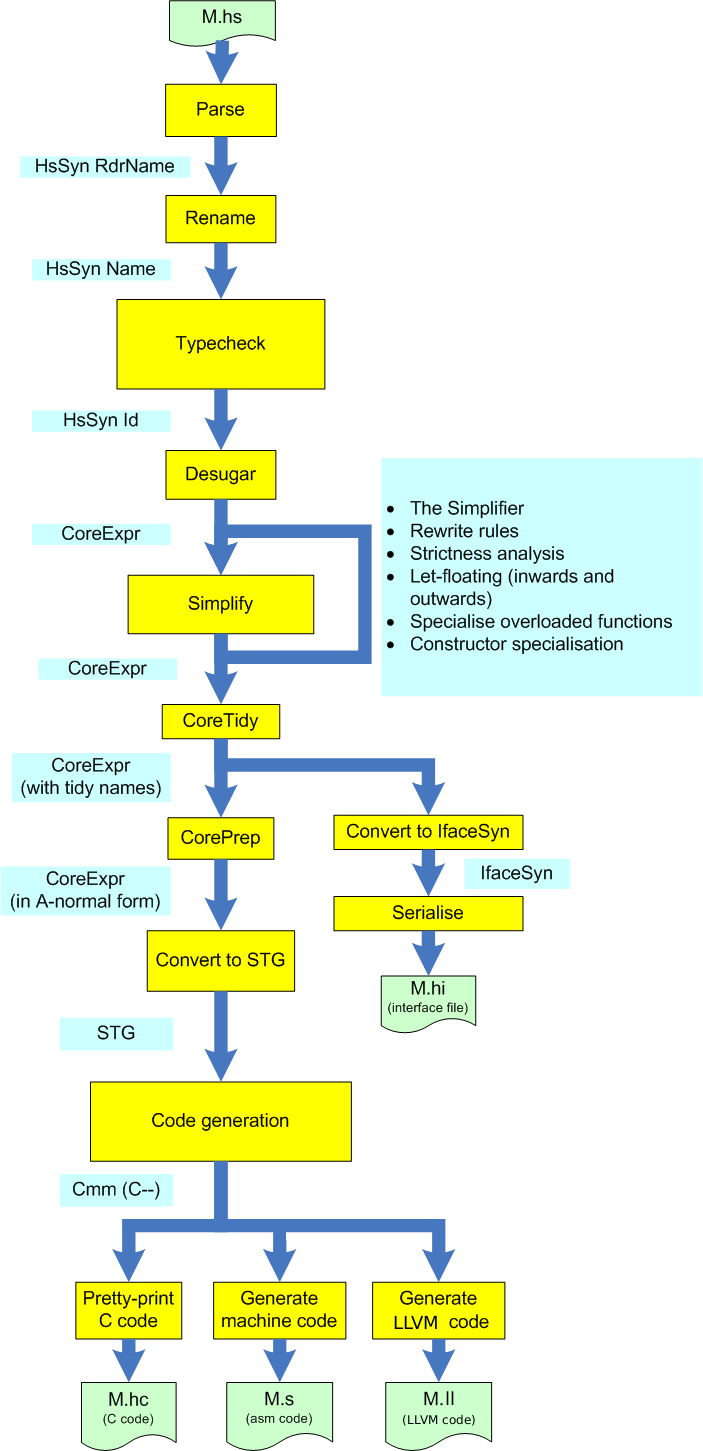
\includegraphics[scale=0.3]{HscPipe2.png}
\end{center}
\caption{The compiler phases}
\label{f:pipeline}
\end{figure}

\subsubsection{Parsing}

We start in the traditional way with parsing, which takes as input a
Haskell source file and produces as output abstract syntax.  In GHC
the abstract syntax datatype @HsSyn@ is parameterised by the types of
the identifiers it contains, so an abstract syntax tree has type
@HsSyn t@ for some type of identifiers @t@.  This enables us to add
more information to identifiers as the program passes through the
various stages of the compiler, while reusing the same type of
abstract syntax trees.

The output of the parser is an abstract syntax tree in which the
identifiers are simple strings, which we call @RdrName@.  Hence, the
abstract syntax produced by the parser has type @HsSyn RdrName@.

GHC uses the tools @Alex@ and @Happy@ to generate its lexical analysis
and parsing code respectively, which are analogous to the tools @lex@
and @yacc@ for C.

GHC's parser is purely functional.  In fact, the API of the GHC
library provides a pure function called @parser@ that takes a @String@
(and a few other things) and returns either the parsed abstract syntax or an
error message.

\subsubsection{Renaming}

Renaming is the process of resolving all of the itentifiers in the
Haskell source code into fully-qualified names, at the same time
identifying any out-of-scope identifiers and flagging errors
appropriately.

In Haskell it is possible for a module to re-export an identifier that
it imported from another module.  For example, suppose module @A@
defines a function called @f@, and module @B@ imports module @A@ and
re-exports @f@.  Now, if a module @C@ imports module @B@, it can refer
to @f@ by the name @B.f@ - even though @f@ is originally defined in
module @A@.  This is a useful form of namespace manipulation; it means
that a library can use whatever module structure it likes internally,
but expose a nice clean API via a few interface modules that re-export
identifiers from the internal modules.

The compiler however has to resolve all this, so that it knows what
each name in the source code corresponds to.  We make a clean
distinction between the \emph{entities}, the ``things themselves'' (in
our example, @A.f@), and the names by which the entities can be
referred to (e.g. @B.f@).  At any given point in the source code,
there are a set of entities in scope, and each may be known by one or
more different names.  The job of the renamer is to replace each of
the names in the compiler's internal representation of the code by a
reference to a particular entity.  Sometimes a name can refer to
several different entities: by itself that is not an error, but if the
name is actually used, then the renamer will flag an ambiguity error
and reject the program.

Renaming takes Haskell abstract syntax (@HsSyn RdrName@) as input, and
also produces abstract syntax as output (@HsSyn Name@).  Here a @Name@
is a reference to a particular entity.

%  More about the
% datatypes that represent names in Section~\ref{s:names}.

Resolving names is the main job of the renamer, but it performs a
plethora of other tasks too: collecting the equations of a function
together and flagging an error if they have differing numbers of
arguments; rearranging infix expressions according to the fixity of
the operators; spotting duplicate declarations; generating warnings
for unused identifiers, and so on.

\subsubsection{Typechecking}

Type checking, as one might imagine, is the process of checking that
the Haskell program is type-correct.  If the program passes the type
checker, then it is guaranteed to not crash at runtime.\footnote{The
  term ``crash'' here has a formal definition that includes hard
  crashes like ``segmentation fault'', but not things like
  pattern-matching failure.  The non-crash guarantee can be subverted
  by using certain unsafe language features, such as the Foreign
  Function Interface.}

The input to the type-checker is @HsSyn Name@ (Haskell source with
qualified names), and the output is @HsSyn Id@.  An @Id@ is a @Name@
with extra information: notable a \emph{type}.  In fact, the Haskell
syntax produced by the type checker is fully decorated with type
information: every identifier has its type attached, and there is
enough information to reconstruct the type of any subexpression
(which might be useful for an IDE, for example).

In practice, type checking and renaming may be interleaved, because
the Template Haskell feature generates code at runtime that itself
needs to be renamed and typechecked.

\subsubsection{Desugaring, and the Core language}

Haskell is a rather large language, containing many different
syntactic forms.  It is intended to be easy for humans to read and
write - there is a wide range of syntactic constructs which gives the
programmer plenty of flexibility in choosing the most appropriate
construct for the situation at hand.  However, this flexibility means
that there are often several ways to write the same code: for example,
an @if@ expression is identical in meaning to a @case@ expression with
@True@ and @False@ branches, and list-comprehension notation can be
translated into calls to @map@, @filter@, and @concat@.  In fact, the
definition of the Haskell language defines all these constructs by
their translation into simpler constructs; the constructs that can be
translated away like this are called ``syntactic sugar''.

It is much simpler for the compiler if all the syntactic sugar is
removed, because the subsequent optimisation passes that need to work
with the Haskell program have a smaller language to deal with.  The
process of desugaring therefore removes all the syntactic sugar,
translating the full Haskell syntax into a much smaller language that
we call \Core{}.  We'll talk about \Core{} in detail in Section~\ref{s:core}.

\subsubsection{Optimisation}

Now that the program is in \Core{}, the process of optimisation
begins.  One of GHC's great strengths is in optimising away layers of
abstraction, and all of this work happens at the \Core{} level.
\Core{} is a tiny functional language, but it is a tremendously
flexible medium for expressing optimisations, ranging from the very
high level, such as strictness analysis, to the very low-level, such
as strength reduction.

Each of the optimisation passes takes \Core{} and produces
\Core{}.  The main pass here is called the \emph{Simplifier}, whose job
it is to perform a large collection of correctness-preserving
transformations on the program, with the goal of producing a more
efficient program.  Some of these transformations are simple and
obvious, such as eliminating dead code or reducing a case expression
when the value being scrutinised is known, and some are more involved,
such as function inlining and applying rewrite rules (Section~\ref{s:rules}).

The simplifier is normally run between the other optimisation passes,
of which there are about six; which passes are actually run and in
which order depends on the optimisation level selected by the user.

\subsubsection{Code Generation}

Once the \Core{} program has been optimised, the process of code
generation begins.  After a couple of administrative passes, the code
takes one of two routes: either it is turned into \emph{byte code} for
execution by the interactive interpreter, or it is passed to the
\emph{code generator} for eventual translation to machine code.

The code generator first converts the \Core{} into a language called
@STG@, which is essentially just \Core{} annotated with more
information required by the code generator.  Then, @STG@ is translated
to @Cmm@, a low-level imperative language with an explicit stack. From
here, the code takes one of three routes:

\begin{itemize}
\item \textbf{Native code generation}: GHC contains simple native code
  generators for a few processor architectures.  This route is fast,
  and generates reasonable code in most cases.

\item \textbf{LLVM code generation}: The @Cmm@ is converted to LLVM
  code and passed to the LLVM compiler.  This route can produce
  significantly better code in some cases, although it takes longer
  than the native code generator.

\item \textbf{C code generation}: GHC can produce ordinary C code.
  This route produces signficantly slower code than the other two
  routes, but can be useful for porting GHC to new platforms.
\end{itemize}

\section{Key design choices}

In this section we focus on a handful of the design choices that have
been particularly effective in GHC.

\subsection{The intermediate language}
\label{s:core}

\newcommand{\clift}[1]{\lfloor#1\rfloor}
\newcommand{\ol}[1]{\overline{#1}}
\newcommand{\tcase}[2]{\mathbf{case}\;#1\;\mathbf{of}\;\ol{#2}}
\newcommand{\tlet}[4]{\mathbf{let}\;#1{:}#2 = #3\;\mathbf{in}\;#4}
\newcommand{\tcast}[2]{#1\xspace\triangleright\xspace#2}
\begin{figure}
$$
\begin{array}{lrll}
\multicolumn{3}{l}{\text{Expressions}} \\
t,e,u & ::= & x  & \text{Variables} \\
      & \mid & K & \text{Data constructors} \\ 
      & \mid & k & \text{Literals} \\
      & \mid & \lambda x{:}\sigma @.@ e \mid e\;u 
             & \text{Value abstraction and application} \\ 
    & \mid   &  \Lambda a{:}\eta @.@ e \mid e\;\phi
             & \text{Type abstraction and application} \\ 
    & \mid    & \mathbf{let}\;\ol{x:\tau = e}\;\mathbf{in}\;u 
             & \text{Local bindings} \\ 
    & \mid    & \tcase{e}{p \to u} 
             & \text{Case expressions} \\ 
    & \mid    & \tcast{e}{\gamma}         &  \text{Casts} \\
    & \mid    & \clift{\gamma}            &  \text{Coercions} \\[2mm] 
 p  & ::=     & K\; \ol{c{:}\eta}\;\;\ol{x{:}\tau} & \text{Patterns} \\[3mm]
\end{array} 
$$
\label{fig:core-syntax}
\caption{The syntax of \Core{}}
\end{figure}

A typical structure for a compiler for a statically-typed language is
this: the program is typechecked, and transformed to some
\emph{untyped} intermediate language, before being optimised.
GHC is different: it has a \emph{statically-typed intermediate language}.
As it turns out, this design choice has had a pervasive effect on the design and development of GHC.

GHC's intermediate language is called \Core{} (when thinking of the
implementation) or System FC (when thinking about the theory).  Its
syntax is given in Figure~\ref{fig:core-syntax}.  The exact details
are not imortant here; the intersted reader can consult
\citet{sulzmann-et-al:fc} for more details.  For our present purposes, however,
the following points are the key ones:
\begin{itemize}
\item Haskell is a very large source language.  The data type representing its syntax tree has literally hundreds of constructors. 

In contrast \Core{} is a tiny, principled, lambda calculus.  It has
extremely few syntactic forms, yet we can translate all of Haskell into \Core{}.

\item Haskell is an \emph{implicitly-typed} source language.  A program may have few or no type annotations; instead it is up to the type inference algorithm to figure out the type of every binder and sub-expressions.  This type inference algorithm is complex, and occasionally somewhat \emph{ad-hoc}, reflecting the design compromises that every real programming language embodies.

In contrast \Core{} is an \emph{explicitly-typed} language.  Every binder has an explicit type, and terms include explicit type abstractions and applications.  \Core{} enjos a very simple, fast type checking algorithm, that checks that the program is type correct.  The algorithm is entirely straightforward; there are no \emph{ad-hoc} compromises.
\end{itemize}
All of GHC's analysis and optimisation passes work on \Core{}. This is
great: because \Core{} is such a tiny language an optimisation has
only a few cases to deal with.  Although \Core{} is small, it is
extremely expressive --- System F was, after all, originally developed
as a foundational calculus for typed computation.
When new language features
are added to the source language (and that happens all the time!) the
changes are usually restricted to the front end; \Core{} stays
unchanged, and hence so does most of the compiler.

But why is \Core{} typed?  After all, if the type inference engine
accepts the source program, that program is presumably well typed, and
each optimisation pass presumably maintains that type-correctness.
\Core{} may enjoy a fast type checking algorithm, but why
would you ever want to run it?  Moreover, making \Core{} typed carries
significant costs, because every transformation or optimisation pass
must produce a well-typed program, and generating all those type
annotations is often non-trivial.

Nevertheless, it has been huge win to have an explicitly-typed intermediate language, for several reasons:
\begin{itemize}
\item Running the \Core{} type checker (we call it \Lint{}) is a very powerful consistency check on the compiler itself.  Imagine that you write an ``optimisation'' that accidentally generates code that treats an integer value as a function, and tries to call it.  The chances are that the program will segmentation fault, or fail at runtime in a bizarre way. Tracing a seg-fault back to the particular optimisation pass that broke the program is a long road.

Now imagine instead that we run \Lint{} after every optimisation pass (and we do, if you use the flag @-dcore-lint@):
it will report a precisely-located error immediately after the
offending optimsiation.  What a blessing.  

Of course, type soundness is not the same as correctness: \Lint{} will
not signal an error if you ``optimise'' $(x*1)$ to $1$ instead of to
$x$.  But if the program passes \Lint{}, it will guarantee to run without seg-faults; and moreover in practice we have found that it is surprisingly hard to accidentally write optimisations that are type-correct but not semantically correct!

\item The type inference algorithm for Haskell is very large and very
      complex: a glance at Figure~\ref{f:lines} confirms that the type
      checker is by far the largest single component of GHC.  Large
      and complex means error-prone.  But \Lint{} serves as an 100\%
      independent check on the type inference engine: if the type
      inference engine accepts a program that is not, in fact,
      type-corect, \Lint{} will reject it. So \Lint{} serves as a 
      powerful auditor of the type inference engine.

\item The existence of \Core{} has also proved to be a tremendous
      sanity check on the \emph{design} of the source language.  Our
      users constantly suggest new features that they would like in
      the language. Sometimes these features are manifestly
      ``syntactic sugar'', convenient new syntax for something you can
      do already. But sometimes they are deeper, and it can be hard to
      tell how far-reaching the feature is.

\Core{} gives us a precise way to evaluate such features.  If the
feature can readily be translated into \Core{}, that reassures us that
nothing fundamentally new is going on: the new feature is syntactic-sugar-like. On the other hand, if it would require an extension to \Core, then we think much, much more carefully.  
\end{itemize}

In practice \Core{} has been incredibly stable: over a 20-year time period we have added exactly one new major feature to \Core{} (namely coercions and their associated casts).  Over the same period, the source languaage has evolved enormously.
We attribte this stability not to our own brilliance, but rather to the fact that \Core{} is based dirctly on foundational mathematics: bravo Girard!


\subsection{Typechecking the source language}

One interesting design decision is whether type-checking should be
done before or after desugaring.  The trade-offs are these:
\begin{itemize}
\item Typechecking before desugaring means that the type checker
must deal directly with Haskell's very large syntax, so the typechecker
has many cases to consider.  If we desugared into (an untyped variant of) \Core{} first, 
one might hope that the type checker would become much smaller.
\item On the other hand, typechecking after desugaring would impose a significant
new obligation: that desugaring does not affect which programs are type-correct.
After all, desugaring implies a deliberate loss of information.
It is probably the case that in 95\% of the cases there no problem, but
\emph{any} problem here would force some compromise in the design of \Core{} to
preserve some extra information. 
\item Most seriously of all, typechecking a desugared program would make it
much harder to report errors that relate to the original program text, and not
to its (sometimes elaborate) desugared version.
\end{itemize}
Most compilers typecheck after desugaring, but for GHC made the opposite choice:
we typecheck the full original Haskell syntax, and then desugar the result.
It sounds as if adding a new syntactic construct might be complicated, but
(following the French school) we have structured the type inference engine in
a way that makes it easy. Type inference is split into two parts: 
\begin{enumerate}
\item Constraint generation: walk over the source syntax tree, generating 
a collection of type constraints.  This step deals with the full syntax of Haskell,
but it is very straightforward code, and it is easy to add new cases.
\item Constraint solving: solve the gathered constraints.  This is where the
subtlety of the type inference engine lies, but it is independent of the source
language syntax, and would be the same for a much smaller or much larger language.
\end{enumerate}
On the whole, the typecheck-before-desugar design choice has turned
out to be a big win.  Yes, it adds lines of code to the typechecker,
but they are \emph{simple} lines. It avoids giving two conflicting
roles to the same data type, and makes the type inference engine
less complex, and easier to modify. Moreover, GHC's type error messages are
pretty good.

\subsection{No Symbol Table}

Compilers usually have one or more data structures known as
\emph{symbol tables}, which are mappings from symbols (e.g.\ variables)
to some information about the variable, such as its type, or where in
the source code it was defined.

In GHC we use symbol tables quite sparingly; mainly in the renamer and
type checker.  As far as possible, we use an alternative strategy: a
variable is a data structure that \emph{contains} all the information
about itself.  Indeed, a large amount of information is reachable by
traversing the data structure of a variable: from a variable we can
see its type, which contains type constructors, which contain their
data constructors, which themselves contain types, and so on.  
For example, here are some 
data types from GHC (heavily abbreviated and simplified):
\begin{code}
  data Id      = MkId Name Type
  data Type    = TyConApp TyCon [Type]
               | ....
  data TyCon   = AlgTyCon Name [DataCon]
               | ...
  data DataCon = MkDataCon Name Type ...
\end{code}
An @Id@ contains its @Type@.  A @Type@ might be an application of a type 
constructor to some arguments (e.g. @Maybe Int@), in which case it contains
the @TyCon@.  A @TyCon@ can be an algebraic data type, in which case it includes
a lits of its data constructors.  Each @DataCon@ includes its @Type@, which of course
mentions the @TyCon@.   And so on.
The whole structure is highly interconnected.  Indeed it is cyclic; for example,
a @TyCon@ may contain a @DataCon@ which contains a @Type@, which contains the
very @TyCon@ we started with.

This approach has some advantages and disadvantages:

\begin{itemize}
\item Many queries that would require a lookup in a symbol table are
  reduced to a simple field access, which is great for efficiency and
  code clarity.
\item There is no need to carry around extra symbol tables, the
  abstract syntax tree already contains all the information.
\item The space overheads are better: all instances of the same
  variable share the same data structure, and there is no space needed
  for the table.
\item The only difficulties arise when we need to \emph{change} any of
  the information associated with a variable.  This is where a symbol
  table has the advantage: we would just change the entry in the
  symbol table.  In GHC we have to traverse the abstract syntax tree
  and replace all the instances of the old variable with the new one;
  indeed the simplifier does this regularly, as it needs to update
  certain optimisation-related information about each variable.
\end{itemize}

It is hard to know whether it would be better or worse overall to use
symbol tables, because this aspect of the design is so fundamental
that it is almost impossible to change.  Still, avoiding symbol tables
is a natural choice in the purely functional setting, so it seems
likely that this approach is a good choice for Haskell.

% %    + we can make circular references easily in Haskell; this would not
% %      be possible without circular references.

\subsection{Inter-module optimisation}

Functional languages encourage the programmer to write small definitions.
For example, here is the definition of @&&@ from the standard library:
\begin{code}
(&&) :: Bool -> Bool -> Bool
True && True = True
_    && _    = False
\end{code}
If every use of such a function really required a function call, efficency
would be terrible.  One solution is to make the compiler treat certain
functions specially; another is to use a pre-processor to replace a ``call''
with the desired inline code.  All of these solutions are unsatisfactory in
one way or another, especially as another solution is so obvious: simply
inline the function.  To ``inline a function'' means to replace the call
by a copy of the function body, suitably instantiating its parameters.

In GHC we have systematically adopted this approach \cite{inlining}.
Virtually nothing is built into the compiler.  Instead, we define as
much as possible in libraries, and use aggressive inlining to elimiate
the overheads.  This means that \emph{programmers can define their own
  libraries that will be inlined and optimised as well as the ones tha
  come with GHC}.

A consequence is that GHC must be able to do cross-module, and indeed
cross-package, inlining.  The idea is simple:
\begin{itemize}
\item When compiling a Haskell module @Lib.hs@, GHC produces object code
in @Lib.o@ and an ``interface file'' in @Lib.hi@.  This interface file
contains information about all the functions that @Lib@ exports, including
both their types and, for sufficiently small functions, their definitions.
\item When compiling a module @Client.hs@ that imports @Lib@, GHC reads the
interface @Lib.hi@.  So if @Client@ calls a function @Lib.f@ defined in @Lib@,
GHC can use the information in @Lib.hi@ to inline @Lib.f@.
\end{itemize}
By default GHC will expose the definition of a function in the
interface file only if the function is ``small'' (there are flags to
control this size threshold).  But we also support an INLINE pragma, to
instruct GHC to inline the definition
agreessively at call sites, regardless of size, thus:
\begin{code}
foo :: Int -> Int 
{-# INLINE foo #-}
foo x = <some big expression>
\end{code}
Cross-module inlining is absolutely essential for defining super-efficient
libraries, but it does come with a cost.  If the author 
upgrades his library, it is not enough to re-link @Client.o@ with the 
new @Lib.o@, because @Client.o@ contains inlined fragments of the old
@Lib.hs@, and they may well not be compatible with the new one.
Another way to say this is that the ABI (Application Binary Interface)
of @Lib.o@ has changed in a way that requires recompilation of its clients.

In fact, the only way for compilation to generate code with a fixed,
predictable, ABI is to disable cross-module optimisation, and this is
typically too high a price to pay for ABI compatibility.  Users
working with GHC will usually have the source code to their entire
stack available, so recompiling is not normally an issue (and, as we
will describe later, the package system is designed around this mode
of working).  However, there are situations where recompiling is not
practical: distributing bug fixes to libraries in a binary OS
distribution, for example.  In the future we hope it may be possible
to find a compromise solution that allows retaining ABI compatibility
while still allowing some cross-module optimisation to take place.

\section{Extensibility}

It is often the case that a project lives or dies according to how
extensible it is.  A monolithic piece of software that is not
extensible has to do everything and do it right, whereas an extensible
piece of software can be a useful base even if it doesn't provide all
the required functionality out of the box.

Open source projects are of course extensible by definition, in that
anyone can take the code and add their own features.  But modifying
the original source code of a project maintained by someone else is
not only a high-overhead approach, it is also not conducive to sharing
your extension with others.  Therefore successful projects tend to
offer forms of extensibility that do not involve modifying the core
code, and GHC is no exception in this respect.

\subsection{User-defined rewrite rules}
\label{s:rules}

The core of GHC is a long sequence of optimisation passes, each of
which performs some semantics-preserving transformormation, \Core{}
into \Core{}.  But the author of a library defines functions that
often have some non-trivial, domain-specific transformations of their
own, ones that cannot possibly be predicted by GHC. So GHC allows
library authors to define \emph{rewrite rules} that are used
to rewrite the program during optimisation \cite{pj-et-al:playing-by-the-rules}.
In this way, programmers
can, in effect, extend GHC with domain-specific optimisations.

One example is the @foldr@/@build@ rule, which is expressed like this:
\begin{code}
{-# RULES "fold/build"    
    forall k z (g::forall b. (a->b->b) -> b -> b) . 
       foldr k z (build g) = g k z
 #-}
\end{code}
The entire rule is a pragma, introduce by ``@{-# RULES@''.  
The rule says that whenever GHC sees the expression @(foldr k z (build g))@
it should rewrite it to @(g k z)@.  This transformation is
semantics-preserving, but it takes a research paper to argue that it
is \cite{gill:short-cut}, so there is no chance of GHC performing it automatically.
Together with a handful of other rules, and
some INLINE pragmas, GHC is able to fuse together list-transforming functions.
For example, the two loops in @(map f (map g xs))@ are fused into one.

Although rewrite rules are simple and easy to use, they have proved to
be a very powerful extension mechanism.  When we first introduced
the feature into GHC, ten years ago, we expected it to be an
occasionally-useful facility.  But in practice it has turned out to be
useful in very many libraries, whose efficiency often depends
crucially on rewrite rules.  For example, GHC's own @base@ library
contains upward of 100 rules, while the popular @vector@ library uses
several dozen.

\subsection{Compiler plugins}

One way in which a compiler can offer extensibility is to allow
programmers to write a pass that is inserted dirctly into the 
compiler's pipeline.  Such passes are often called ``plugins''.
GHC supports plugins in the following way:
\begin{itemize}
\item The programmer writes a \Core{} to \Core{} pass, as an ordinary
Haskell function in a module @P.hs@, say,
and compiles it to object code.  
\item When compiling some module, the programmer uses the command-line 
flag @-plugin P@.  (Alternatively, he can give the flag in a pragma
at the start of the module.)
\item GHC searches for @P.o@, dynamically links it into the running
GHC binary, and calls it at the appropriate point in the pipeline
\end{itemize}
But what is ``the appropriate point in the pipeline''?  GHC does not know,
and so it allow the plugin to make that decision.  As a result of this and
other matters, the API that the plugin must offer is a bit more complicated
than a single \Core{} to \Core{} function --- but not much.  

Plugins sometimes require, or produce, auxiliary plugin-specific data. 
For example, a plugin might perform some analysis on the functions in the
module being compiled (@M.hs@, say), 
and might want to put that information in the interface file @M.hi@, so that
the plugin has access to that information when compiling modules that import @M@.
GHC offers an annotation mechanism to support this.

Plugins and annotations are relatively new to GHC.  They have a higher
barrier to entry than rewrite rules, because the plugin is
manipulating GHC's internal data structures, but of course they can do
much more.  It remains to be seen how widely they will be used.


\subsection{GHC as a library: the GHC API}
\label{s:ghcapi}

One of GHC's original goals was to be a \emph{modular} foundation that
others could build on.  We wanted the code of GHC to be as transparent
and well-documented as possible, so that it could be used as the basis
for research projects by others; we imagined that people would want to
make their own modifications to GHC to add new experimental features
or optimisations.  Indeed, there have been some examples of this: for
example, there exists a version of GHC with a Lisp front-end, and a
version of GHC that generates Java code, both developed entirely
separately by individuals with little or no contact with the GHC team.

However, producing modified versions of GHC represents only a small
subset of the ways in which the code of GHC can be re-used.  As the
popularity of the Haskell language has grown, there has been an
increasing need for tools and infrastructure that understand Haskell
source code, and GHC of course contains a lot of the functionality
necessary for building these tools: a Haskell parser, abstract syntax,
type checker and so on.

With this in mind, we made a simple change to GHC: rather than
building GHC as a monolithic program, we build GHC as a
\emph{library}, that is then linked with a small \emph{Main} module to
make the GHC executable itself, but also shipped in library form so
that users can call it from their own programs.  At the same time we
built an API to expose GHC's funcionality to clients.  The API
provides enough functionality to implement the GHC batch compiler and
the GHCi interactive environment, but it also provides access to
individual passes such as the parser and type checker, and allows the
data structures produced by these passes to be inspected.  This change
has given rise to a wide range of tools built using the GHC API,
including:

\begin{itemize}
\item A documentation tool,
\emph{Haddock}\footnote{\url{http://www.haskell.org/haddock/}}, which
reads Haskell source code and produces HTML documentation
\item New versions of the GHCi front end with additional features,
e.g. \emph{ghci-haskeline}\footnote{\url{http://hackage.haskell.org/package/ghci-haskeline}} which was subsequently merged back into GHC,
\item IDEs that offer advanced navigation of Haskell source code,
e.g. \emph{Leksah}\footnote{\url{http://hackage.haskell.org/package/leksah}},
\item \emph{hint}\footnote{\url{http://hackage.haskell.org/package/hint}}, a simpler API for on-the-fly evaluation of Haskell
  source code.
\end{itemize}

\subsection{The Package System}

The package system has been a key factor in the growth in use of the
Haskell language in recent years.  Its main purpose is to enable
Haskell programmers to share code with each other, and as such is an
important aspect of extensibility: the package system extends the
shared codebase beyond GHC itself.

The package system embodies various pieces of infrastructure that
together make sharing code easy.  With the package system as the
enabler, the community has built a large body of shared code; rather
than relying on libraries from a single source, Haskell programmers
draw on libraries developed by the whole community.  This model has
worked well for other languages: CPAN for Perl for example, although
Haskell being a predominantly compiled rather than interpreted
language presents a somewhat different set of challanges.

Basically, the package system lets a user manage libraries of Haskell
code written by other people, and use them in their own programs and
libraries.  Installing a Haskell library is as simple as uttering a
single command, e.g.

\begin{verbatim}
$ cabal install zlib
\end{verbatim}

\noindent downloads the code for the @zlib@ package from
@http://hackage.haskell.org@, compiles it using GHC, installs the
compiled code somewhere on your system (e.g.\ in your home directory
on a Unix system), and registers the installation with GHC.
Furthermore, if @zlib@ depends on any other packages that are not yet
installed, those will also be downloaded, compiled and installed
automatically before @zlib@ itself is compiled.  It is a tremendously
smooth way to work with libraries of Haskell code shared by others.

The package system is made of four components, only the first of which
is strictly part of the GHC project:

\begin{itemize}
\item Tools for managing the \emph{package database}, which is simply
  a repository for information about the packages installed on your
  system.  GHC reads the package database when it starts up, so that
  it knows which packages are available and where to find them.

\item A library called @Cabal@ (Common Architecture for Building
  Applications and Libraries), which implements functionality for
  building, installing and registering individual packages.

\item A website at @http://hackage.haskell.org@ which hosts packages
  written and uploaded by users.  The website automatically builds
  documentation for the packages which can be browsed online.  At the
  time of writing, Hackage is hosting over 3000 packages covering
  functionality including database libraries, web frameworks, GUI
  toolkits, data structures, and networking.

\item The @cabal@ tool which ties together the Hackage website and the
  @Cabal@ library: it downloads packages from Hackage, resolves
  dependencies, and builds and installs packages in the right order.
  New packages can also be uploaded to Hackage using @cabal@ from the
  command line.
\end{itemize}

These components have been developed over several years by members of
the Haskell community and the GHC team, and together they make a
system that fits perfectly with the Open Source development model.
There are no barriers to sharing code or using code that others have
shared (provided you respect the relevant licenses, of course).  You
can be using a package that someone else has written literally within
seconds of finding it on Hackage.

Hackage has been so successful that the remaining problems it has are
now those of scale: users find it difficult to choose amongst the four
different database frameworks, for example.  Ongoing developments are aimed
at solving these problems in ways that leverage the community.  For
example, allowing users to comment and vote on packages will make it
easier to find the best and most popular packages, and collecting data
on build success or failures from users and reporting the results will
help users avoid packages that are unmaintained or have problems.

% ---------------------------------------------
\section{The Runtime System}
\label{s:rts}

The Runtime System (hereafter, the RTS) is a library of mostly C code
that is linked into every Haskell program.  It provides the support
infrastructure needed for running the compiled Haskell code, including
the following main components:

\begin{itemize}
\item Memory management, including a parallel, generational, garbage collector;
\item Thread management and scheduling;
\item The primitive operations provided by GHC;
\item A bytecode interpreter and dynamic linker for GHCi.
\end{itemize}

The rest of this section is divided into two: first we focus on a
couple of the aspects of the design of the RTS that we consider to
have been successful and instrumental in making it work so well, and
secondly we talk about the coding practices and infrastructure we have
built in the RTS for coping with what is a rather hostile programming
environment.

\subsection{Key design decisions}

In this section we describe two of the design decisions in the RTS
that we consider to have been particularly successful.

\subsubsection{The block layer}

The garbage collector is built on top of a \emph{block layer} that
manages memory in units of blocks, where a block is a multiple of 4KB
in size.  The block layer has a very simple API:

\begin{verbatim}
typedef struct bdescr_ {
    void *               start;
    struct bdescr_ *     link;
    struct generation_ * gen;   // generation
    // .. various other fields
} bdescr;

bdescr * allocGroup (int n);
void     freeGroup  (bdescr *p);
bdescr * Bdescr     (void *p);  // a macro
\end{verbatim}

This is the only API used by the garbage collector for allocating and
deallocating memory.  Blocks of memory are allocated with @allocGroup@
and freed with @freeGroup@.  Every block has a small structure
associated with it called a \emph{block descriptor} (@bdescr@).  The
operation @Bdescr(p)@ returns the block descriptor associated with an
arbitrary address @p@; this is purely an address calculation based on
the value of @p@ and compiles to a handful of arithmetic and
bit-manipulation instructions.

Blocks may be linked together into chains using the @link@ field of
the @bdescr@, and this is the real power of the technique.  The
garbage collector needs to manage several distinct areas of memory
such as \emph{generations}, and each of these areas may need to grow
or shrink over time.  By representing memory areas as linked lists of
blocks, the GC is freed from the difficulties of fitting multiple
resizable memory areas into a flat address space.

The implementation of the block layer uses techniques that are
well-known from C's @malloc()/free()@ API: it maintains lists of free
blocks of various sizes, and coalesces free areas.  The operations
@freeGroup()@ and @allocGroup()@ are carefully designed to be O(1).

One major advantage of this design is that it needs very little
support from the OS, and hence is great for portability.  The block
layer needs to allocate memory in units of 1MB, aligned to a 1MB
boundary.  While none of the common OSs provide this functionality
directly, it is implementable without much difficulty in terms of the
facilities they do provide.  The payoff is that GHC has no dependence
on the particular details of the addresss-space layout used by the OS,
and it coexists peacefully with other users of the address space, such
as shared libraries and operating system threads.

There is a small up-front complexity cost for the block layer, in
terms of managing chains of blocks rather than contiguous memory.
However, we have found that this is a cost is more than repaid in
flexibility and portabilty; for example, the block layer enabled a
particularly simple algorithm for parallel GC to be implemented
\cite{parallel-gc}.

\subsubsection{Lightweight threads and parallelism}

We consider concurrency to be a vitally important programming
abstraction, particularly for building applications like web servers
that need to interact with large numbers of external agents
simultaneously.  If concurrency is an important abstraction, then it
should not be so expensive that programmers are forced to avoid it, or
build elaborate infrastructure to amortise its cost (e.g.\ thread
pools).  We believe that concurrency should just work, and be cheap
enough that you don't worry about forking threads for small tasks.

All operating systems provide threads that work perfectly well, the
problem is that they are far too expensive.  Typical OSs struggle to
handle thousands of threads, whereas we want to manage threads by the
million.

Green threads, otherwise known as ligthweight threads or user-space
threads, are a well-known technique for avoiding the overhead of
operating system threads.  The idea is that threads are managed by the
program itself, or a library (in our case, the RTS), rather than by
the operating system.  Managing threads in user space should be
cheaper, because fewer traps into the operating system are required.

In the GHC RTS we take full advantage of this idea.  A context switch
only occurs when the thread is at a \emph{safe point}, where very
little additional state needs to be saved.  Because we use accurate
GC, the stack of the thread can be moved and expanded or shrunk on
demand.  Contrast these with OS threads, where every context switch
must save the entire processor state, and where stacks are immovable
so a large chunk of address space has to be reserved up front for
each thread.

Green threads can be vastly more efficient than OS threads, so why
would anyone want to use OS threads?  It comes down to three main
problems:

\begin{itemize}
\item Blocking and foreign calls.  A thread should be able to make a
  call to an OS API or a foreign library that blocks, without blocking
  all the other threads in the system.

\item Parallelism.  Threads should automatically run in parallel if
  there are multiple processor cores on the system.

\item Some external libraries (notably OpenGL and some GUI libraries)
  have APIs that must be called from the same OS thread each time,
  because they use thread-local state.
\end{itemize}

It turns out that all of these are difficult to arrange with green
threads.  Nevertheless, we persevered with green threads in GHC and
found solutions to all three:

\begin{itemize}
\item When a Haskell thread makes a foreign call, another OS thread
  takes over the execution of the remaining Haskell threads \cite{concffi04}.  A small
  pool of OS threads are maintained for this purpose, and new ones are
  created on demand.

\item GHC's scheduler multiplexes many lightweight Haskell threads
  onto a few heavyweight OS threads; it implements a transparent M:N
  threading model.  Typically N is chosen to be the same as the number
  of processor cores in the machine, allowing real parallelism to take
  place but without the overhead of having a full OS thread for each
  lightweight Haskell thread.

  In order to run Haskell code, an OS thread must hold a
  \emph{Capability}\footnote{we have also called it a ``Haskell
    Execution Context'', but the code currently uses the Capability
    terminology}: a data structure that holds the resources required
  to execute Haskell code, such as the nursery (memory where new
  objects are created).  Only one OS thread may hold a given
  Capability at a time.

\item We provide an API for creating a \emph{bound thread}: a Haskell
  thread that is tied to one specific OS thread, such that any foreign
  calls made by this Haskell thread are guaranteed to be made by that
  OS thread.
\end{itemize}

So in the vast majority of cases, Haskell's threads behave exactly
like OS threads: they can make blocking OS calls without affecting
other threads, and they run in parallel on a multicore machine.  But
they are orders of magnitude more efficient, in terms of both time and
space.

Having said that, the implementation does have one problem that users
occasionally run into, especially when running benchmarks.  We
mentioned above that lightweight threads derive some of their
efficiency by only context-switching at ``safe points'', points in the
code that the compiler designates as safe, where the internal state of
the virtual machine (stack, heap, registers etc.) is in a tidy state
and garbage collection could take place.  In GHC, a safe point is
whenever memory is allocated; which in almost all Haskell programs
happens regularly enough that the program never executes more than a
few tens of instructions without hitting a safe point.  However, it is
possible in highly optimised code to find loops that run for many
iterations without allocating memory.  This tends to happen often in
benchmarks (e.g.\ functions like factorial and fibonacci).  It occurs
less often in real code, although it does happen.  The lack of safe
points prevents the scheduler from running, which can have detrimental
effects.  It is possible to solve this problem, but not without
impacting the performance of these loops, and often people care about
saving every cycle in their inner loops.  This may just be a
compromise we have to live with.

\section{Developing GHC}

GHC is a single project with a twenty-year life span, and is still in
a ferment of innovation and development.  For the most part our 
infrastructure and tooling has been conventional.  For example, we use
a bug tracker (Trac), a wiki (also Trac), and use Git for revision
control. (This revision-control mechanism evolved from purely manual,
then CVS, then Darcs, before finally moving to Git in 2010.)  There 
are a few points that may be less universal, and we offer them here.

\subsection{Comments and notes}

One of the most serious difficulties in a large, long-lived project is 
keeping technical documetation up to date.  We have no silver bullet,
but we offer one low-tech mechanism that has served us particularly well: @Notes@.

When writing code, there is often a moment when a careful programmer
will mentally say something like ``This data type has an important
invariant''.  She is faced with two choices, both unsatisfactory.  She
can add the invariant as a comment, but that can make the data type
declaration too long, so that it is hard to see what the constructors
are.  Alternatively , she can document the invariant elsewhere, and
risk it going out of date.  Over twenty years, \emph{everything} goes out of
date!

Thus motivated, we developed the following very simple convention:
\begin{itemize}
\item Comments of any significant size are not interleaved with code,
but instead set off by themselves, with a heading in standard form, thus:
\begin{code}
  Note [Equality-constrained types]
  ~~~~~~~~~~~~~~~~~~~~~~~~~~~~~~~~~
  The type   forall ab. (a ~ [b]) => blah
  is encoded like this:

     ForAllTy (a:*) $ ForAllTy (b:*) $
     FunTy (TyConApp (~) [a, [b]]) $
     blah
\end{code}
\item A the point where the comment is relevant, we add a short comment
referring to the Note:
\begin{code}
 data Type
   = FunTy Type Type
	-- See Note [Equality-constrained types]

   | ...
\end{code}
The comment highlights that something interesting is going on, and gives
a precise reference to the comment that explains.  It sounds trivial, but
the precision is vastly better than our previous habit of saying ``see the comment above'', 
because it often was not clear \emph{which} of the many comments above was intended,
and after a few years the comment was not even above (it was below; or gone altogether).
\end{itemize}
Not only is it possible to go from the code that refers to the @Note@
to the @Note@ itself, but the reverse is also possible, and that is often
useful.  Moreover, the same @Note@ may be referred to from multiple points
in the code.

This simple, ASCII-only technique, with no automated support, has
transformed our lives: GHC has around 800 @Notes@, and the number
grows daily.

\subsection{How to keep on refactoring}

The code of GHC is churning just as quickly, if not more so, than it
was ten years ago.  There is no doubt that the complexity of the
system has increased manyfold over that same time period: we saw
measures of the amount of code in GHC earlier.  Yet, the system
remains manageable.  We attribute this to three main factors:

\begin{itemize}
\item There's no substitute for good software engineering.  Modularity
  always pays off: making the APIs between components as small as
  possible makes the individual components more flexible because they
  have fewer interdependencies.  For example, GHC's \Core datatype
  being small reduces the coupling between Core-to-Core passes, to the
  extent that they are almost completely independent and can be run in
  an arbitrary order.

\item Developing in a strongly-typed language makes refactoring a
  breeze.  Whenever we need to change a data type, or change the
  number of arguments or type of a function, the compiler immediately
  tells us what other places in the code need to be fixed.  Simply
  having an absolute guarantee that a large class of errors have been
  statically ruled out saves a huge amount of time, especially when
  refactoring.  It is scary to imagine how many hand-written test
  cases we would need to provide the same level of coverage that the
  type system provides.

\item When programming in a purely functional language, it is
  hard to introduce accidental dependencies via state.  If you decide
  that you suddenly need access to a piece of state deep in an
  algorithm, in an imperative language you might be tempted to just
  make the state globally visible rather than explicitly pass it down
  to the place that needs it.  This way eventually leads to a tangle
  of invisible dependencies, and \emph{brittle code}: code that breaks
  easily when modified.  Pure functional programming forces you to
  make all the dependencies explicit, which exerts some negative
  pressure on adding new dependencies, and fewer dependencies means
  greater modularity.  Certainly when it is \emph{necessary} to add a
  new dependency then purity makes you write more code to express the
  dependency, but in our view it is a worthwhile price to pay for the
  long-term health of the code base.

  As an added benefit, purely functional code is thread-safe by
  construction and tends to be easier to parallelise.
\end{itemize}

% *** How did writing in a (pure) functional language affect the design?
%    - lets us make circular references easily (see data structures)
%
%    - we use mutation heavily in the type checker, but other passes
%      are pure.
%
%    - splittable name supply trick

\subsection{Crime doesn't pay}

Looking back over the changes we've had to make to GHC as it has
grown, a common lesson emerges: being less than purely functional,
whether for the purposes of efficiency or convenience, tends to have
negative consequences down the road.  We have a couple of great
examples of this:

\begin{itemize}
\item GHC uses a few data structures that rely on mutation internally.
  One is the @FastString@ type, which uses a single global hash table;
  another is a global @NameCache@ that ensures all external names are
  assigned a unique number.  When we tried to parallelise GHC (that
  is, make GHC compile multiple modules in parallel on a multicore
  processor), these data structures based on mutation were the
  \emph{only} sticking points.  Had we not resorted to mutation in
  these places, GHC would have been almost trivial to parallelise.

  In fact, although we did build a prototype parallel version of GHC,
  GHC does not currently contain support for parallel compilation, but
  that is largely because we have not yet invested the effort required
  to make these mutable data structures thread-safe.

\item GHC's behaviour is governed to a large extent by command-line
  flags.  These command-line flags are by definition constant over a
  given run of GHC, so in early versions of GHC we made the values of
  these flags available as top-level constants. For example, there was
  a top-level value @opt_GlasgowExts@ of type @Bool@, that governed
  whether certain language extensions should be enabled or not.
  Top-level constants are highly convenient, because their values
  don't have to be explicitly passed as arguments to all the code that
  needs access to them.

  Of course these options are not really \emph{constants}, because
  they change from run to run, and the definition of @opt_GlasgowExts@
  involves calling @unsafePerformIO@ because it hides a side effect.
  Nevertheless, this trick is normally considered ``safe enough''
  because the value is constant within any given run; it doesn't
  invalidate compiler optimisations, for example.

  However, GHC was later extended from a single-module compiler to a
  multi-module compiler.  At this point the trick of using top-level
  constants for flags broke, because the flags may have different
  values when compiling different modules.  So we had to refactor
  large amounts of code to pass around the flags explicitly.

  Perhaps you might argue that treating the flags as \emph{state} in
  the first place, as would be natural in an imperative language,
  would have sidestepped the problem.  To some extent this is true,
  although purely functional code has a number of other behefits, not
  least of which is that representing the flags by an immutable data
  structure means that the resulting code is already thread-safe and
  will run in parallel without modification.
\end{itemize}

\subsection{Developing the RTS}

GHC's runtime system presents a stark contrast to
the compiler in many ways.  There is the obvious difference that the
runtime system is written in C rather than Haskell, but there are also
considerations unique to the RTS that give rise to a different design
philosophy:

\begin{enumerate}
\item Every Haskell program spends a lot of time executing code in the
  RTS: 20--30\% is typical, but characteristics of Haskell
  programs vary a lot and so figures greater or less than this range
  are also common.  Every cycle saved by optimising the RTS is
  multiplied many times over; so it is worth spending a lot of time
  and effort to save those cycles.

\item The runtime system is statically linked into every Haskell
  program\footnote{that is, unless dynamic linking is being used}, so
  there is an incentive to keep it small.

\item Bugs in the runtime system are often inscrutable to the user
  (e.g.\ ``segmentation fault'') and are hard to work around.  For
  example, bugs in the garbage collector tend not to be tied to the
  use of a particular language feature, but arise when some complex
  combination of factors emerges at runtime.  Furthermore, bugs of
  this kind tend to be non-deterministic (only occurring in some
  runs), and highly sensitive (tiny changes to the program make the
  bug disappear).  Bugs in the multithreaded version of the runtime
  system present even greater challenges.  It is therefore worth going
  to extra lengths to prevent these bugs, and also to build
  infrastructure to make identifying them easier.

  The symptoms of an RTS bug are often indistinguishable from two
  other kinds of failure: hardware failure, which is more common than
  you might think, and misuse of unsafe Haskell features like the FFI.
  The first job in diagnosing a runtime crash is to rule out these two
  other causes.

\item The RTS is low-level code that runs on several different
  architectures and operating systems, and is regularly ported to
  new ones.  Portability is important.
\end{enumerate}

Every cycle and every byte is important, but correctness is even more
so.  Moreover, the tasks performed by the runtime system are
ineherently complex, so correctness is hard to begin with.
Reconciling these has lead us to some interesting defensive
techniques, which we describe in the following sections.

\subsubsection{Coping with complexity}
\label{s:rtsbugs}

The RTS is a complex and hostile programming environment.  In contrast
to the compiler, the RTS has almost no type safety.  In fact, it has
even less type safety than most other C programs, because it is
managing data structures whose types live at the Haskell level and not
at the C level.  For example, the RTS has no idea that the object
pointed to by the tail of a cons cell is either @[]@ or another cons:
this information is simply not present at the C level.  Moreover, the
process of compiling Haskell code erases types, so even if we told the
RTS that the tail of a cons cell is a list, it would still have no
information about the pointer in the head of the cons cell.  So the
RTS code has to do a lot of casting of C pointer types, and it gets
very little help in terms of type safety from the C compiler.

So our first weapon in this battle is to \emph{avoid putting code in
  the RTS}.  Wherever possible, we put the minimum amount of
functionality into the RTS and write the rest in a Haskell library.
This has rarely turned out badly: Haskell code is far more robust and
concise than C, and performance is usually perfectly acceptable.
Deciding where to draw the line is not an exact science, although in
many cases it is reasonably clear.  For example, while it might be
theoretically possible to implement the garbage collector in Haskell,
in practice it is extremely difficult because Haskell does not allow
the programmer precise control of memory allocation, and so dropping
down to C for this kind of low-level task makes practical sense.

There is plenty of functionality that can't be (easily) implemented in
Haskell, and writing code in the RTS is not pleasant.  In the next
section we focus on one aspect of managing complexity and correctness
in the RTS: maintaining invariants.

\subsection{Invariants, and checking them}

The RTS is full of invariants.  Many of them are trivial and easy to
check: for example, if the pointer to the head of a queue is @NULL@,
then the pointer to the tail should also be @NULL@.  The code of the
RTS is littered with assertions to check these kinds of things.
Assertions are our go-to tool for finding bugs before they manifest;
in fact, when a new invariant is added, we often add the assertion
before writing the code that implements the invariant.

Some of the invariants in the runtime are far more difficult to
satisfy, and to check.  One invariant of this kind that pervades more
of the RTS than any other is the following: \emph{the heap has no
  dangling pointers}.

Dangling pointers are easy to introduce, and there are many places
both in the compiler and the RTS itself that can violate this
invariant.  The code generator could generate code that creates invalid
heap objects; the garbage collector might forget to update the pointers
of some object when it scans the heap.  Tracking down these kinds of
bugs can be extremely time consuming\footnote{it is, however, one of
  the author's  favourite activities!} because by the time the program eventually
crashes, execution might have progressed a long way from where the
dangling pointer was originally introduced.  There are good debugging
tools available, but they tend not to be good at executing the program
in reverse.\footnote{recent versions of GDB and the Microsoft Visual Studio debugger do have some support for reverse execution, however.}

The general principle is: \emph{if a program is going to crash, it
  should crash as soon, as noisily, and as often as
  possible.}\footnote{This quote comes from the GHC coding style
  guidelines, and was originally written by Alastair Reid, who worked
  on an early version of the RTS.}

The problem is, the no-dangling-pointer invariant is not something
that can be checked with a constant-time assertion.  The assertion
that checks it must do a full traversal of the heap!  Clearly we
cannot run this assertion after every heap allocation, or every time
the GC scans an object (indeed, this would not even be enough, as
dangling pointers don't appear until the end of GC, when memory is
freed).

So, the debug RTS has an optional mode that we call \emph{sanity
  checking}.  Sanity checking enables all kinds of expensive
assertions, and can make the program run many times more slowly.  In
particular, sanity checking runs a full scan of the heap to check for
dangling pointers (amongst other things), before \emph{and} after
every GC.  The first job when investigating a runtime crash is to run
the program with sanity checking turned on; sometimes this will catch
the invariant violation well before the program actually crashes.

% \subsubsection{Debugging the multithreaded RTS}
% 
% \SDM{If we're after squashing ``Developing the RTS'' a bit, then
%   nuking this section would be my first choice.}
% 
% GHC supports parallel and concurrent execution of Haskell programs,
% and contains its own thread scheduler.  In fact, in many ways the GHC
% RTS is a small operating system.
% 
% GHC comes with both single-threaded and multithreaded variants of the
% RTS.  Concurrent Haskell programs run perfectly well with the
% single-threaded RTS: the RTS scheduler runs the Haskell threads in
% round-robin fashion on its one and only OS thread.  The only downside
% to doing this is that when one Haskell thread is making a foreign
% call, no other Haskell threads can run until the foreign call returns.
% The mulitthreaded RTS relaxes this restriction: when a Haskell thread
% makes a foreign call, another OS thread takes over the execution of
% the other Haskell threads in the system.  In fact, there can be
% multiple OS threads running Haskell threads at the same time, which is
% the only way for concurrent or parallel programs to achieve a speedup
% on a multi-core machine.
% 
% Diagnosing and fixing failures in the multithreaded RTS presents
% some significant challenges.  If we're lucky, inspecting the state of
% the RTS internals in the debugger at the time of the crash is enough
% to diagnose the bug, but if not, things are much more difficult:
% 
% \begin{itemize}
% \item First, it is often impossible to provoke the failure
%   deterministically.  To provoke the failure we may have to run the
%   program many times.
% 
% \item Therefore, our usual tricks for going back in time, such as
%   stopping at the GC just before the failure, don't work.
% 
% \item Sanity checking can be useful, but sometimes this distorts the
%   execution profile of the program sufficiently that the bug stops
%   manifesting.
% \end{itemize}
% 
% Perhaps our most potent tool is assertions: if the crash indicates
% that some invariant has been violated, we add assertions to check the
% invariant at more places in the code, and hope to narrow down the
% cause of the failure that way.
% 
% Sometimes that isn't enough, and we need more insight into what the
% program was doing shortly before it crashed.  The RTS of course can
% produce copious amounts of debugging output, organised into different
% classes and selectable by flags at runtime.  However, this turns out
% to be less than useful for finding bugs in multithreaded programs: the
% act of generating the debugging output slows down the program and adds
% synchronisation, which often stops the bug from manifesting.
% 
% This is where GHC's \emph{event logging} infrastructure comes in
% handy: the RTS can log events in a binary format, using per-thread
% buffers to avoid synchronisation.  This feature was added primarily
% for profiling---the outpout is used by our parallel profiler
% \emph{ThreadScope}---but it turns out to be invaluable for debugging,
% too.

% \section{Retrospective}

% \subsection{C is not a good target language}

% - Getting good performance while targetting C is too hard
%   - tail calls
%   - registers
%   - shadow stack
%
% - Compiling via C is slow
%
% - Portability: C is good here, but LLVM is better now
%
% - Compiling to LLVM is better, but still not quite a perfect fit:
%   LLVM wants to manage the stack, we have to avoid that.
%
% - Native back end compiles quickly, but generates mediocre code
%   (perfectly acceptable for most programs)

% \subsection{Lazy evaluation}

% *** How did _laziness_ affect the design
%
%    - The native code generator is lazy: code is generated as it is
%      written to the output file, not all at once (saves a lot of
%      space, native code is much bigger than Cmm)
%        - BUT, this property is easy to break, we have done so several
%          times, and we now have a regression test for it.
%
%    - laziness is used to read in and typecheck interface files on demand
%      (is this a *good* design??)
%
%    - finding space leaks is tricky: we have lots of strict fields and
%      explicit seqing of data structures between passes (and these
%      data structures are *deep*, see description of data structures).
%

% \subsection{What would we do differently?}

%    - Generic traversals (maybe).



%
% \section{Data structures}
% \label{s:data}
% 
% \subsection{FastString}
% 
% %   - standard atom-like string storage, with one twist:
% %   - UTF-8 encoded, cached mapping to Z-encoding
% 
% \subsection{Names, names, and names}
% \label{s:names}
% 
% %   Tell the story about names: OccName, RdrName, Name, Id
% 
% \subsection{HsSyn: abstract syntax for Haskell}
% 
% % Abstract syntax parameterised over names
% %   So that typecheck/rename can use the same data type for input and output
% 
% \subsection{Entities: TyCon, DataCon, Class, Id}
% 

% \section{Libraries}

% We have to include in the source distribution, and ship, libraries
% that GHC depends on.
%
%  - we need to be able to bootstrap GHC from a single source tree
%  - we want to offload development effort for key libraries,
%    but benefit from them in GHC itself (containers, bytestring)
%
% But this means that
%
%  - making local changes is difficult
%  - we have to comply with the licenses
%  - it's a big deal to add a dependency on a new library
%  - upgrading these libraries later is hard, because the GHC package
%    depends on the old one.

% \section{Bootstrapping}

% Interesting things to say about bootstrapping?
%  - sometimes a released GHC has a bug, which only shows up later and
%    we have to work around it (e.g. the 7.2.1 case-floating bug)

% \section{Tools and development practices}

% Greg said they only want this kind of stuff if it is different and
% interesting.
%
% * build systems?  How does bootstrapping make things interesting?
% (2 or 3-stage build, now built into the build system, originally
% needed separate trees).
%
%    * non-recursive make, previously: Imake, plain GNU make.
%
% * Validate?

\section{Conclusion}

GHC has consumed a significant portion of the authors' lives over the
last 20 years, and we are rather proud of how far it has come.  It is
not the only Haskell implementation, but it is the only one in regular
use by hundreds of thousands of people to get real work done.  We are
constantly surprised when Haskell turns up being used in unusual
places; one recent example is Haskell being used to control the
systems in a garbage
truck\footnote{\url{http://www.haskell.org/pipermail/haskell-cafe/2010-April/075647.html}}.

For many, Haskell and GHC are synonymous: it was never intended to be
so, and indeed in many ways it is counterproductive to have just one
implementation of a standard, but the fact is that maintaining a good
implementation of a programming language is a lot of work.  We hope
that our efforts in GHC to support the standard and to clearly delimit
each separate language extension will make it feasible for more
implementations to emerge and to integrate with the the package system
and other infrastructure.  Competition is good for everyone!

We are deeply indebted to Microsoft in particular for giving us the
opportunity to develop GHC as part of our research and to distribute
it as open source.

\bibliographystyle{abbrvnat}
\bibliography{aos}

\end{document}
